\section{Introduction}

\subsection{Overview}
The following are the three main families of machine learning methods,
which are also the topics of these notes:

\begin{itemize}
    \item Supervised Learning: parametric/non-parametric
          algorithms(e.g.\ nearest neighbors, decision trees and
          random forests), kernel methods, deep neural networks
          (e.g.\ feedforward, convolutional and recurrent networks).
    \item Unsupervised Learning: clustering, dimensionality reduction,
          autoencoders, deep generative models.
    \item Reinforcement Learning: these notes only cover a high-level
          introduction.
\end{itemize}

\vspace{20mm}

\begin{figure}[h]
    \centering
    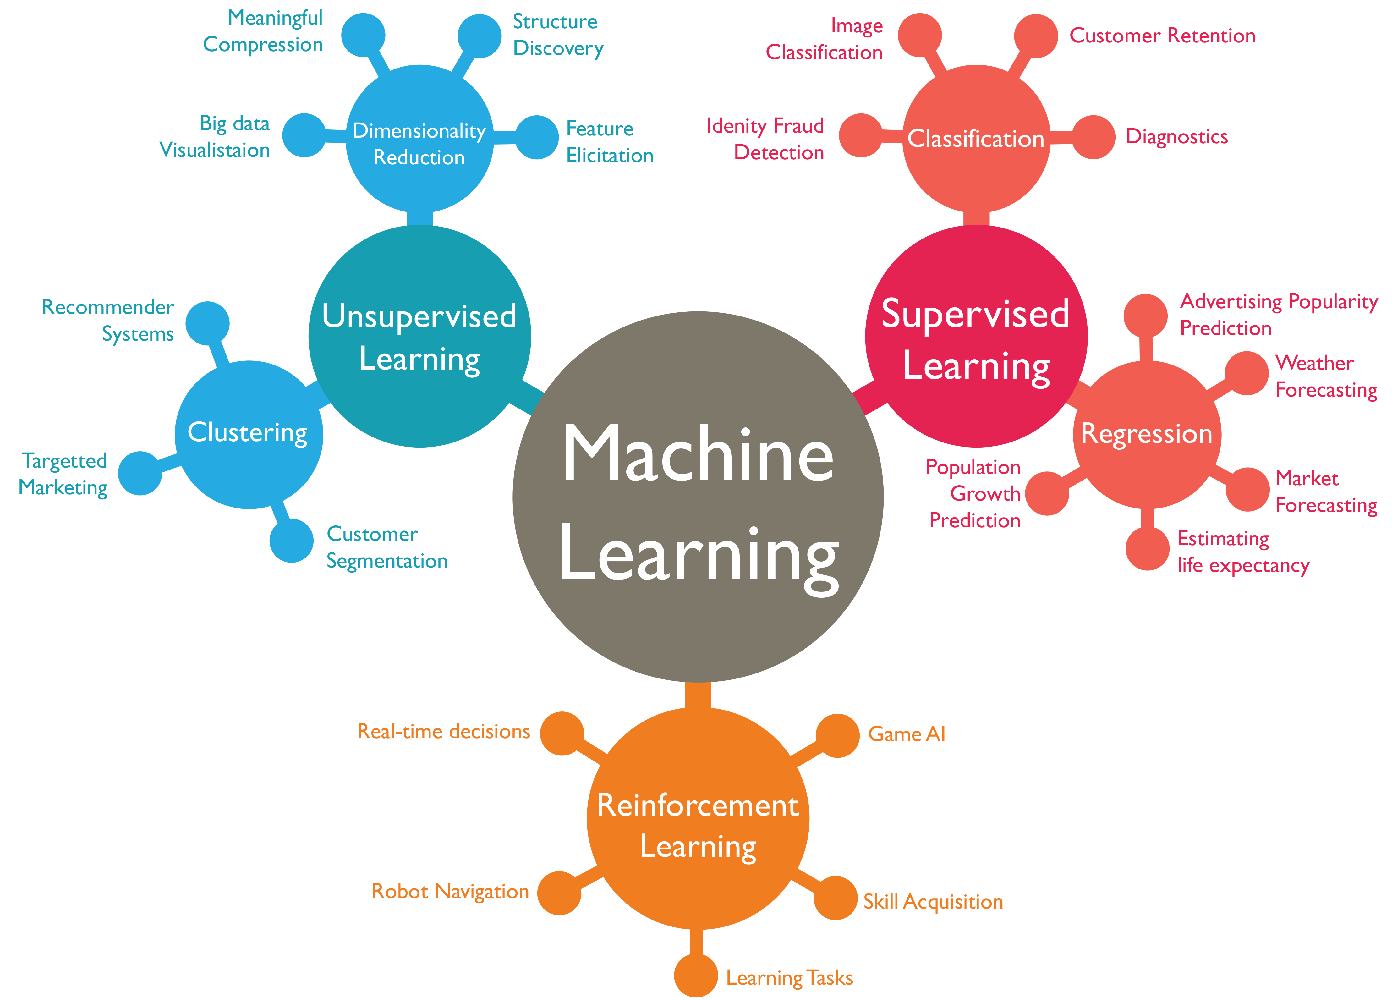
\includegraphics[width=0.56\textwidth]{../img/World_of_ML}
    \caption{High-level description of the world of Machine Learning}
\end{figure}

\subsection{What is Machine Learning?}
There are several definitions of what Machine Learning is, among which
we can find the following that perfectly reflect its conceptual nature:

\vspace{5mm}

\begin{quoting}
    "Machine learning is the study of computer algorithms that improve
    automatically through experience. It is seen as a part of artificial
    intelligence."
\end{quoting}

\hspace{350pt}
\href{https://en.wikipedia.org/wiki/Machine_learning}{--- \underline{Wikipedia}}

\vspace{5mm}

\begin{quoting}
    "Machine learning is the science of getting computers to act without
    being explicitly programmed."
\end{quoting}

\hspace{317pt}
\href{https://en.wikipedia.org/wiki/Arthur_Samuel}{--- \underline{A. Samuel (1959)}}

\vspace{10mm}

Given all these expressive and equivalent definitions, the general idea
of what Machine Learning is and how it differentiates from the
traditional way of programming can be summarized by the following image:

\vspace{10mm}

\begin{figure}[h]
    \centering
    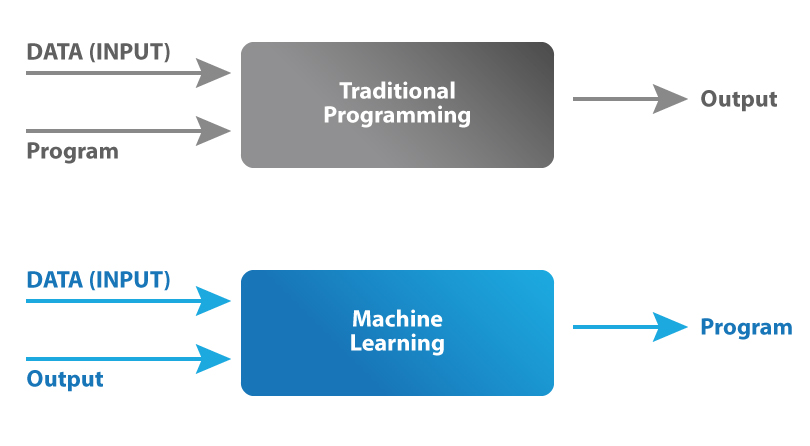
\includegraphics[width=0.56\textwidth]{../img/ML_vs_TP}
    \caption{Machine Learning vs Traditional Programming}
\end{figure}

\vspace{5mm}

By observing the image it becomes clear that in traditional programming
the programmer writes a program and then gives it some input data in
order to produce some output. In machine learning, on the other hand,
the conceptual model is totally different because in this case the
programmer still gives some input data but also gives some known result
(e.g.\ data with annotations/labels), which in combination with the
previous ones are used to produce a program. In this way the machine
learns from the input data and the data with annotations to be able
write a program.

\newpage

Some problems are so hard to solve that it becomes not impossible but
extremely difficult to write programs that solve them and even if such
programs are produced by writing them manually then it is likely that
these programs will not be able to provide sufficiently satisfiable
results. So in these cases it is preferable to make the machine learn
from the data and write the program that will provide some better
results. An excellent example is for instance a robot that has to learn
how to walk because it is extremely difficult to write a suitable
program for this kind of task but it is extremely useful to make the
robot learn from the data because in this way it will also capture the
real-world noise and in general all the unexpected things, which could
not be modelled by a program written manually. Unfortunately there are
many other examples in which the machine learning approach seems to be
the most promising. Nevertheless all the solutions obtained with the
machine learning approach present a common structure, in the sense that
there are always \underline{\emph{three fundamental elements}} which are
the following:

\begin{enumerate}
    \item \emph{\textbf{Data}}: \emph{a lot of data} is required in
          order to build complex and more or less reliable models.
    \item \emph{\textbf{Algorithms}}: there are \emph{a lot of
              algorithms} that can process the data mentioned at the
          point 1, each of which has its own peculiarities. The
          choice of a particular algorithm always depends on the
          task to be addressed.
    \item \emph{\textbf{Model}}: this is the result of applying the
          algorithms mentioned at the point 2 to the data mentioned at
          the point 1, which will be used on future data \emph{similar}
          to the ones that were used for its training. So this result is
          somehow the summary of the knowledge that has been
          extrapolated from the data and represents the so-called
          \emph{"knowledge"} that computers acquire by processing the
          data through the algorithms.
\end{enumerate}

\vspace{5mm}

\begin{figure}[h]
    \centering
    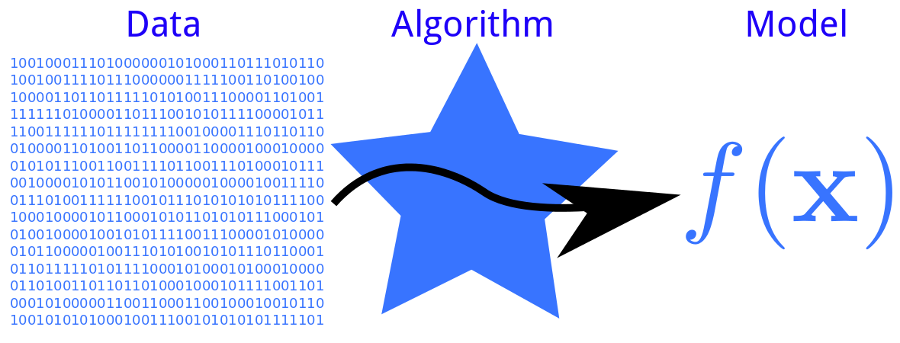
\includegraphics[width=0.8\textwidth]{../img/Data_algorithm_model}
    \caption{Three fundamental elements in Machine Learning}
\end{figure}

\vspace{5mm}

So the main reason why machine learning is so important and so widely
used consists in the \textcolor{orange}{\textbf{Hardness}} of manually
writing programs that should represent satisfiable solutions to a
particular class of problems. This hardness is then instantiated based
on the particular nature of the problem:

\newpage

\begin{itemize}
    \item \textbf{Lack of Expertise}: Human beings have no idea how they
          should program the robot to navigate the surface of Mars
          because until now no human being has had the opportunity to
          explore this planet directly. So it is better for the machine
          to learn what to do autonomously.
    \item \textbf{Lack of Expressiveness}: Sometimes it is too difficult
          to explain the human experience such as sight or hearing and
          so to define a precise set of rules to follow. A great example
          is speech recognition where deducing the person's name from a
          particular waveform becomes significantly complex, therefore
          the best solution is to learn from the data and improve
          performance accordingly.
    \item \textbf{Personalization}: There are situations in which some
          kind of personalization is required and is not feasible for a
          manually written program to provide such personalization to all
          customers. Excellent examples are personalized medicine and the
          recommendations provided by streaming services.
    \item \textbf{Big Data}: In almost all situations in which machine
          learning is used a big amount of data is required for model
          training, but there are some situations in which the amount of
          data to be processed and to be reasoned about in order to
          achieve a particular goal is exceptionally large and therefore
          could not be handled by a manually written program. A great
          example is genomics where the amount of data to be used is
          extremely large.
\end{itemize}

\vspace{5mm}

It should be mentioned though that there are situations in which machine
learning \textbf{is not useful.} Generally this happens when the rule,
which determines how the machine is supposed to act, is perfectly known.
So if the final goal is to calculate a payroll or perform a calculation
using a well-known physical law, then traditional programming is perfect
here.

After having seen the main reasons why machine learning is so widely
used, it is mandatory to mention some of its most important practical
applications:

\begin{itemize}
    \item \textbf{Pattern Recognition}: This classic application
          consists in recognizing patters, which means that, given a
          certain input such as an image of handwritten digits, facial
          identities, facial expressions or a medical image, it is
          possible to recognize certain similarities and continuous
          repetitions of some structures seen before and be able to
          deduce the targeted content of that input. It is useful to
          mention that images are not the only available data type used
          in pattern recognition.
          \vspace{5mm}

          \begin{figure}[h]
              \centering
              \begin{subfigure}{0.3\textwidth}
                  \centering
                  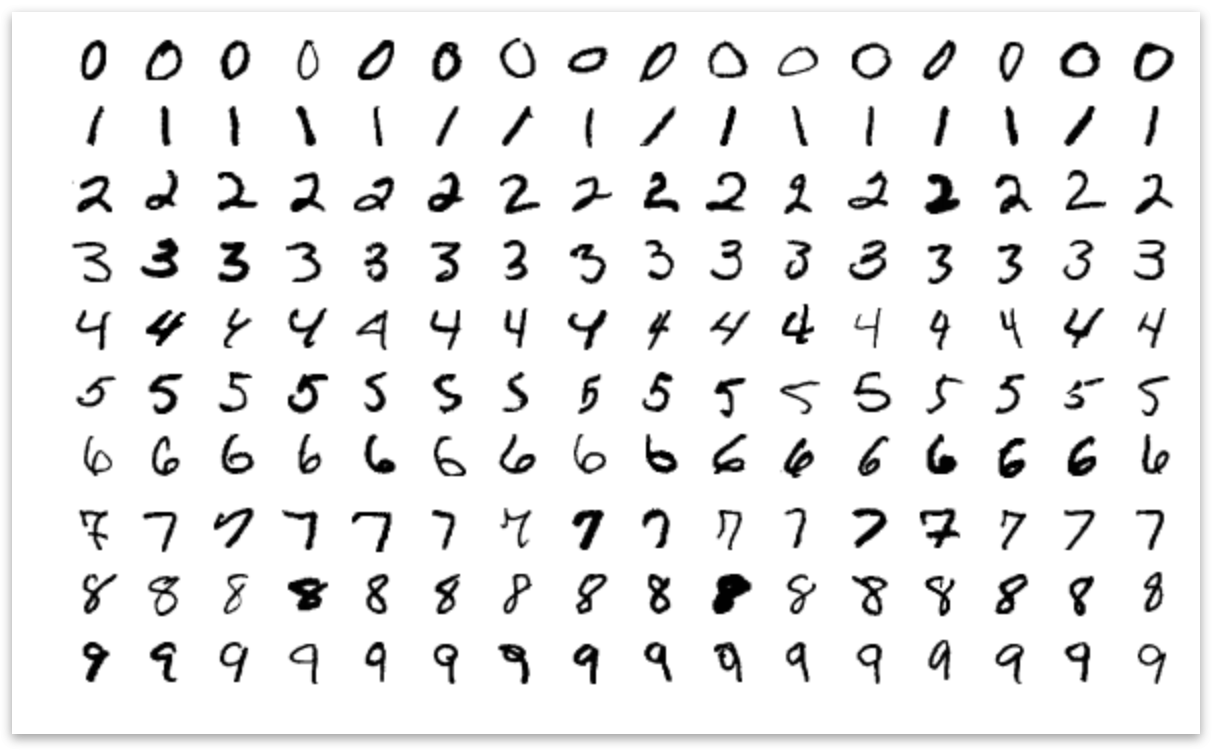
\includegraphics[width=\textwidth]{../img/Handwritten_digits}
              \end{subfigure}
              \hfill
              \begin{subfigure}{0.3\textwidth}
                  \centering
                  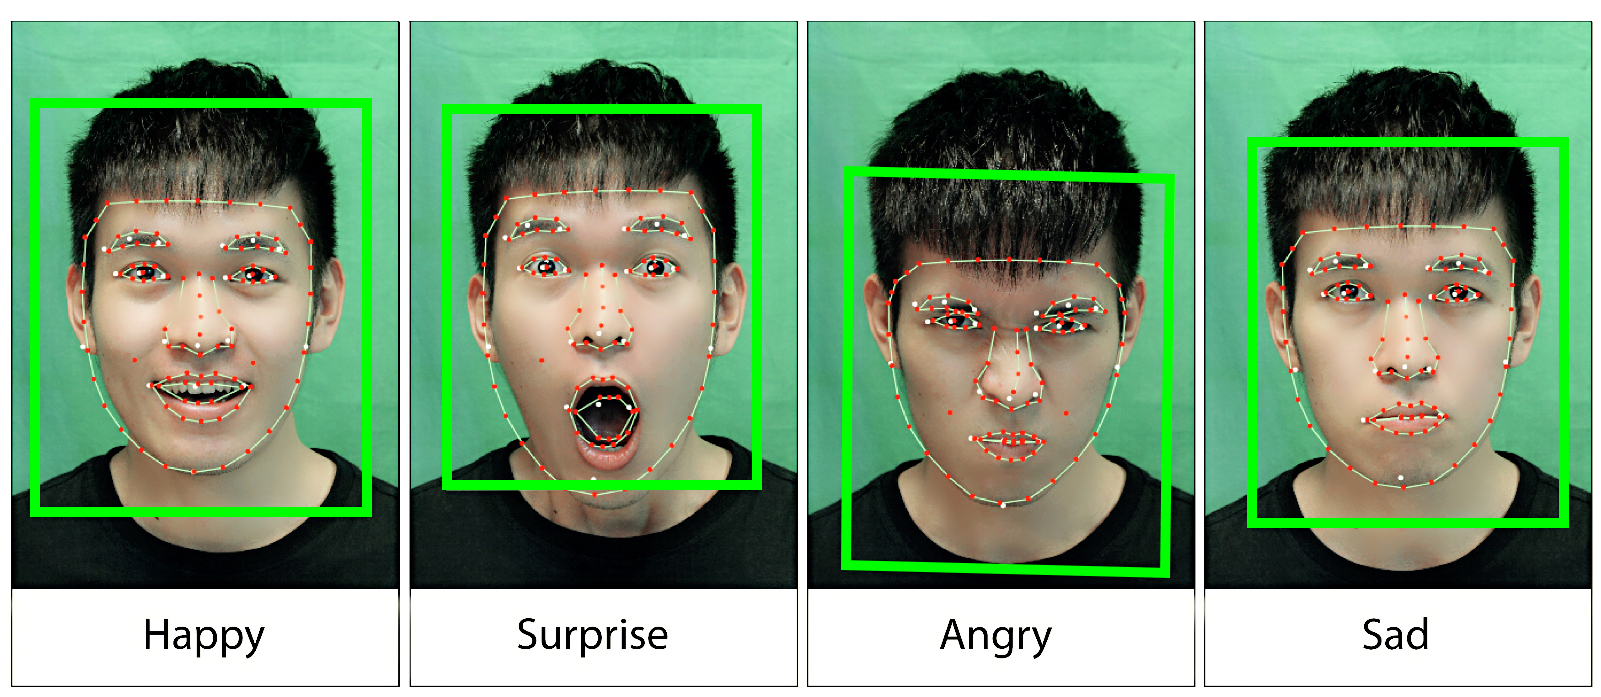
\includegraphics[width=\textwidth, height=0.55\textwidth]{../img/Facial_expr}
              \end{subfigure}
              \hfill
              \begin{subfigure}{0.3\textwidth}
                  \centering
                  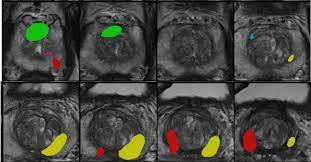
\includegraphics[width=\textwidth]{../img/Medical_img}
              \end{subfigure}
              \caption{Some examples of Pattern Recognition}
          \end{figure}

          \newpage
    \item \textbf{Pattern Generation}: This is another application which
          is extremely used nowadays and consists in generating patterns,
          which means that, given a certain distribution of data to learn
          from, it is possible to produce samples based on these data.
          For example with this technique it is possible to generate
          fake images and artificial motion sequences.
          \vspace{10mm}

          \begin{figure}[h]
              \centering
              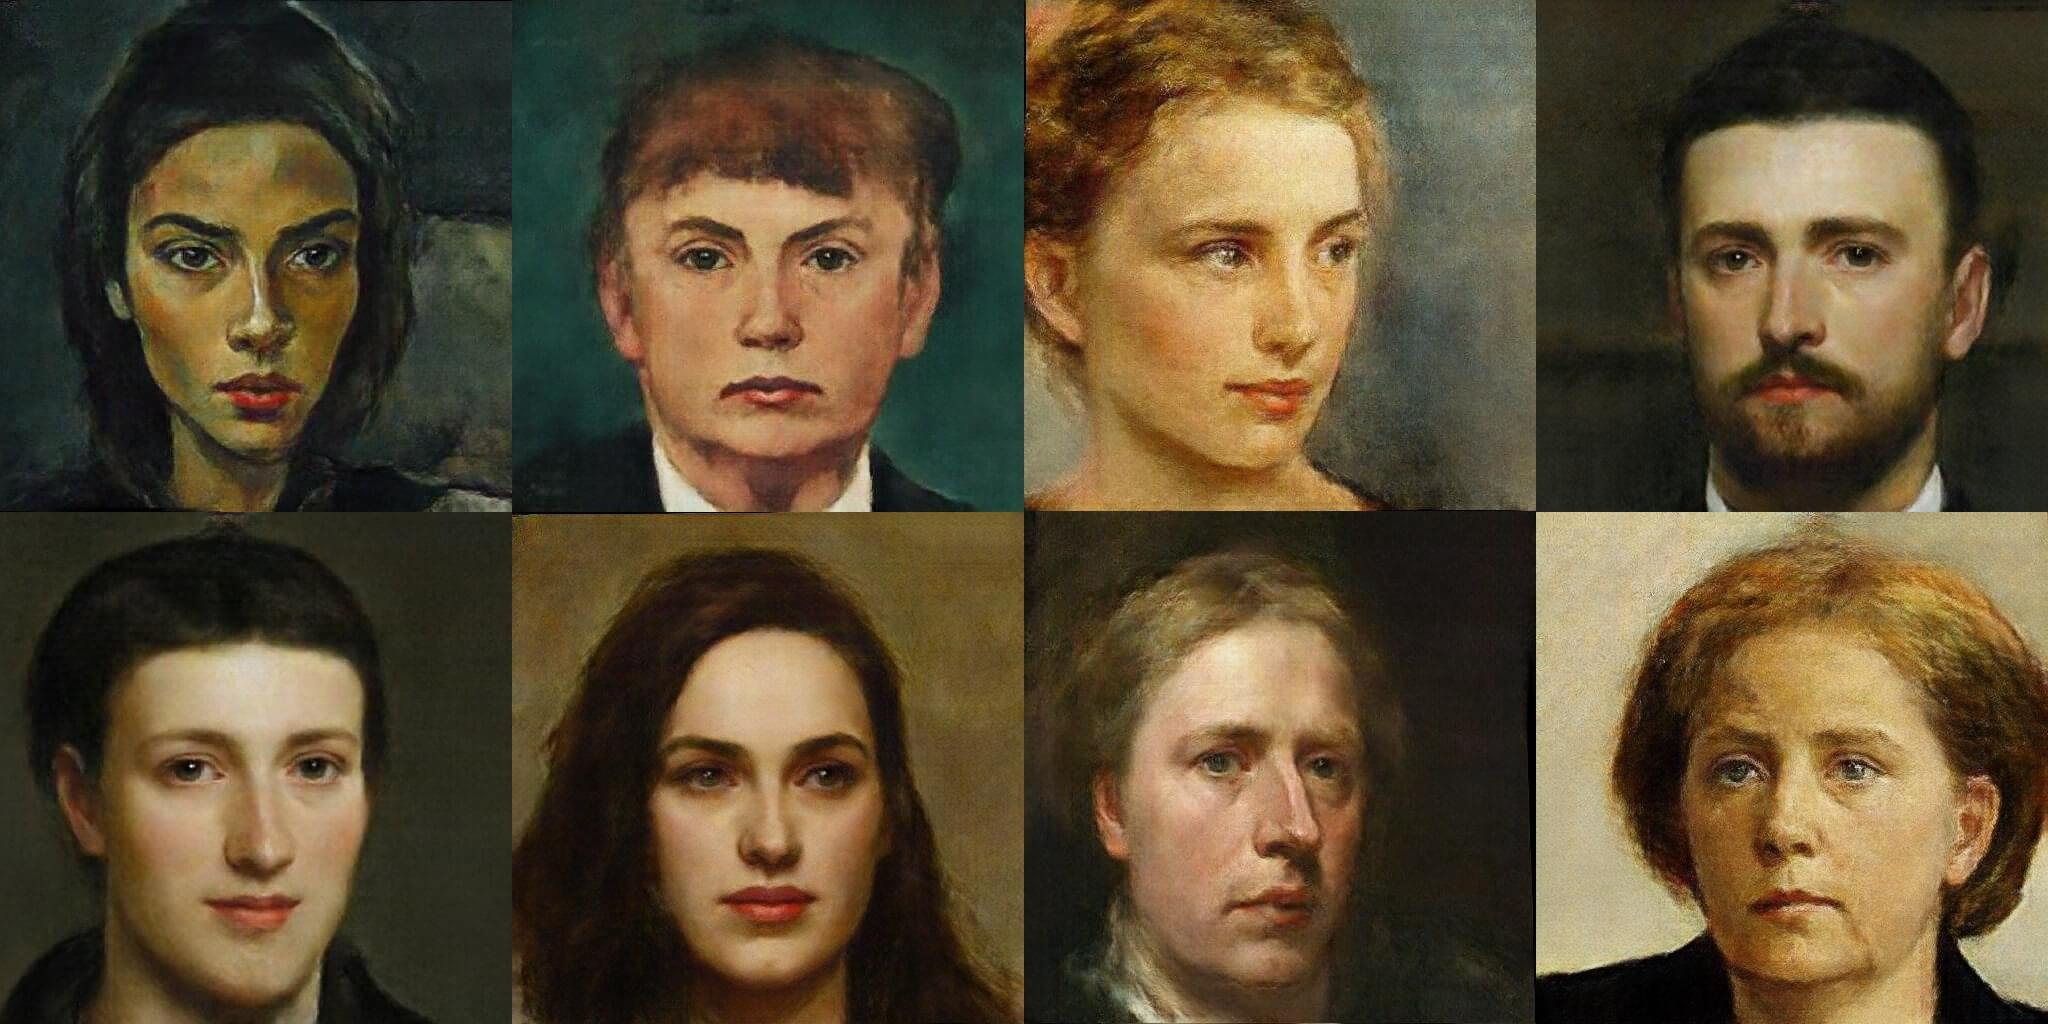
\includegraphics[width=0.7\textwidth]{../img/Fake_img}
              \caption{Some generated portraits of famous people}
          \end{figure}

          \vspace{10mm}
    \item \textbf{Anomaly Detection}: This is another important
          application which consists in detecting anomalies, which means
          that, given a certain amount of data, it is possible to
          produce machine learning models that will be able to predict
          unusual behavior. Some relevant examples are unusual credit
          card transactions, unusual patterns of sensor readings,
          unusual video surveillance frames and unusual system logins.
          \vspace{10mm}

          \begin{figure}[h]
              \centering
              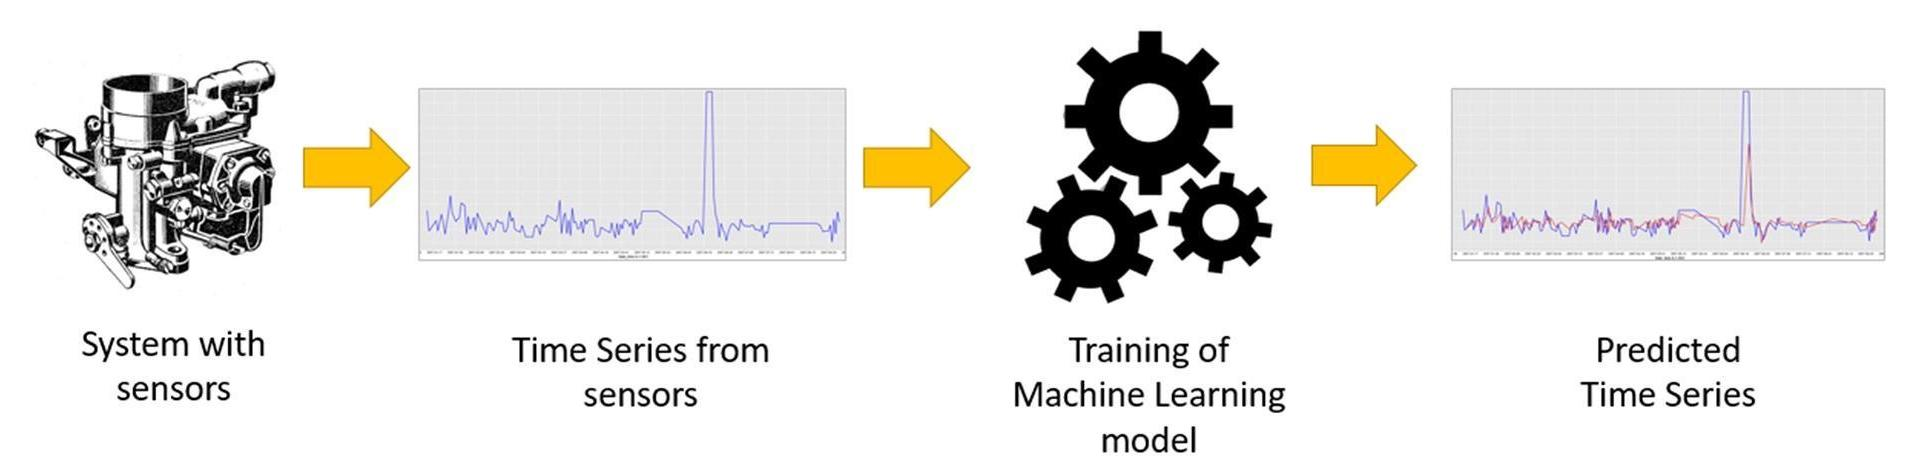
\includegraphics[width=0.9\textwidth]{../img/Anomaly_detect}
              \caption{Anomaly detection in a system with sensors}
          \end{figure}

          \newpage
    \item \textbf{Prediction}: This is an extremely important
          application in finance since it provides predictions on future
          stock prices or currency exchange rates. Nowadays it is also
          used in autonomous driving to predict future moves of people
          and other vehicles and to avoid possible accidents. Moreover,
          it is also used in gaming to predict future best moves, as it
          has been demonstrated by the AlphaGo program developed by the
          Google DeepMind group.
          \vspace{5mm}

          \begin{figure}[h]
              \centering
              \begin{subfigure}{0.45\textwidth}
                  \centering
                  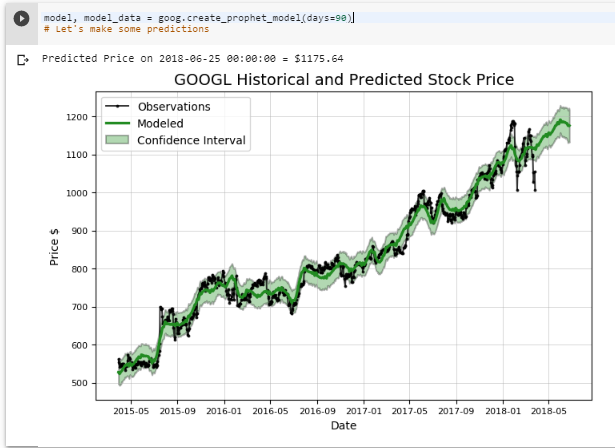
\includegraphics[width=\textwidth]{../img/Prediction_finance}
              \end{subfigure}
              \hfill
              \begin{subfigure}{0.45\textwidth}
                  \centering
                  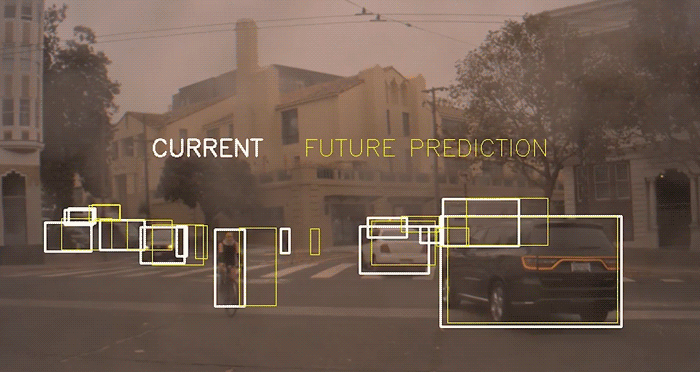
\includegraphics[width=\textwidth]{../img/Autonomous_driving}
              \end{subfigure}
          \end{figure}

          \vspace{5mm}

          \begin{figure}[h]
              \centering
              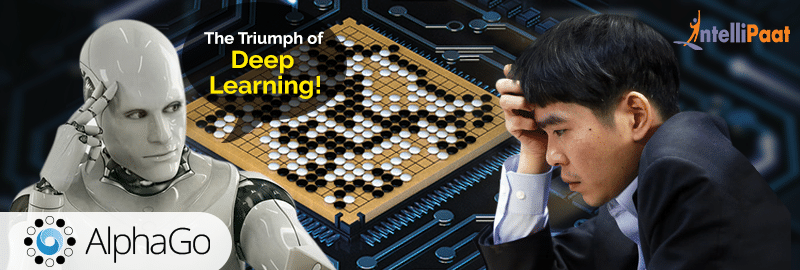
\includegraphics[width=0.9\textwidth]{../img/AlphaGo}
              \caption{Some examples of Prediction}
          \end{figure}

          \vspace{5mm}
\end{itemize}

At this point, it is worth mentioning some other definitions of what
Machine Learning is, provided by some big experts in this field:

\vspace{5mm}

\begin{quoting}
    "It is concerned with the automatic discovery of regularities in
    data through the use of computer algorithms and with the use of
    these regularities to take actions."
\end{quoting}

\hspace{284pt}
\href{https://en.wikipedia.org/wiki/Christopher_Bishop}{--- \underline{Christopher M. Bishop}}

\newpage

\begin{quoting}
    "The goal of machine learning is to develop methods that can
    automatically detect patterns in data, and then to use the uncovered
    patterns to predict future data or other outcomes of interest."
\end{quoting}

\hspace{312pt}
\href{https://www.cs.ubc.ca/~murphyk/}{--- \underline{Kevin P. Murphy}}

\vspace{5mm}

\begin{quoting}
    "Machine learning is about predicting the future based on the past."
\end{quoting}

\hspace{325pt}
\href{https://www.cs.ubc.ca/~murphyk/}{--- \underline{Hal Daume III}}

\vspace{10mm}

Given these last three definitions, it is possible to detect two
fundamental steps of machine learning consisting in automatically
discovering some regularities(i.e.\ patterns) and applying these
regularities to take some actions, such as predicting future data. At
this point, it becomes natural to introduce the typical machine learning
pipeline:

\begin{enumerate}
    \item \emph{\textbf{Training}}: At this stage of the process the
          past knowledge is represented by the so-called \emph{training data},
          which will be passed through a particular \emph{algorithm}
          to produce the so-called \emph{model}, also called
          \emph{predictor}. During this stage, the so-called
          \emph{feature extraction} also takes place, which basically
          consists in extracting from the raw data of the training
          set some kind of representations, called \emph{features},
          which are essential for adequate processing. These features
          will also be used by the aforementioned model to process
          future data.
    \item \emph{\textbf{Testing(Inference)}}: At this stage, on the
          other hand, a component of the future knowledge is represented
          by the so-called \emph{testing data}, which will be passed to
          the \emph{model}, generated during the first stage, to produce
          some \emph{predictions}, which are the other component of the
          future knowledge.
\end{enumerate}

% \vspace{5mm}

\begin{figure}[h]
    \centering
    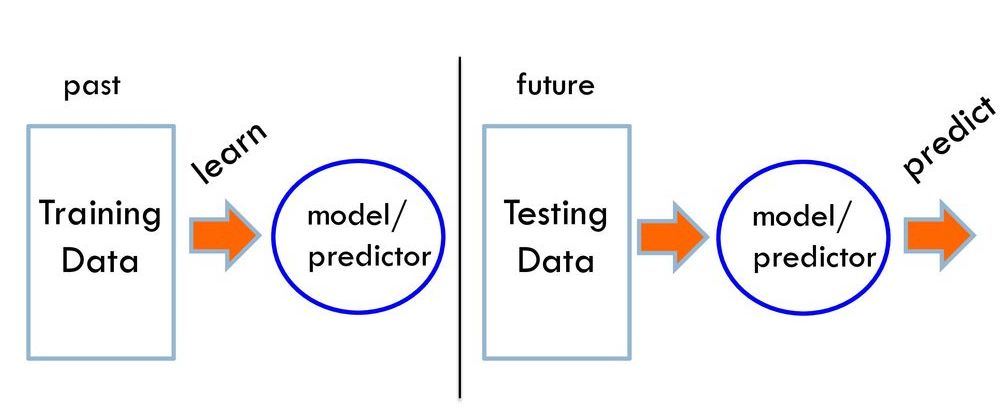
\includegraphics[width=0.85\textwidth]{../img/Typical_ML_process}
    \caption{Typical machine learning process}
\end{figure}

\newpage

The last definition of Machine Learning, which will be seen in this
section and which introduces the concept of performance measure, is the
following:

\vspace{5mm}

\begin{quoting}
    "A computer program is said to learn from \textbf{experience E} with
    respect to some class of \textbf{tasks T} and \textbf{performance
        measure P}, if its performance at tasks in T, as measured by P,
    improves with experience E."
\end{quoting}

\hspace{310pt}
\href{https://en.wikipedia.org/wiki/Tom_M._Mitchell}{--- \underline{T. Mitchell (1970)}}

\vspace{10mm}

Basically what this definition states is that machine learning is the
study of algorithms that:

\begin{itemize}
    \item improve their performance P
    \item at some task T
    \item with experience E
\end{itemize}

\vspace{5mm}

At this point, thanks to this definition, it is possible to describe any
machine learning problem by defining the triplet
$\left\langle T,P,E\right\rangle$,
which is then instantiated based on the particular
nature of the problem:

\begin{itemize}
    \item
          \begin{example}
              T: Recognizing handwritten words.
              P: Percentage of words correctly classified.
              E: Database of human-labeled images of handwritten words.
          \end{example}
    \item
          \begin{example}
              T: Driving on four-lane highways using vision sensors.
              P: Average distance traveled before a human-judged error.
              E: A sequence of images and steering commands recorded
              while observing a human driver.
          \end{example}
    \item
          \begin{example}
              T: Categorize email messages as spam or legitimate.
              P: Percentage of email messages correctly classified.
              E: Database of emails, some with human-given labels.
          \end{example}
\end{itemize}

\vspace{5mm}

Given all these high-level definitions, reasons of usage, practical
applications and some more detailed explanations of the fundamental
elements of machine learning, it is worth mentioning some of the
real-world success stories:

\begin{itemize}
    \item \emph{Face Detection}: The first working system in 2002.
    \item \emph{Pedestrian Detection}: The first working system in 2005.
    \item \emph{Body Tracking(RGB-D)}: Used for example in gaming.
\end{itemize}

\newpage

\subsection{What is Deep Learning?}

In order to understand what Deep Learning is, it should be useful to
observe the image below that represents in chronological order the
popularity growth of Artificial Intelligence and its two most famous
subsets, which are Machine Learning and Deep Learning.

\begin{figure}[h]
    \centering
    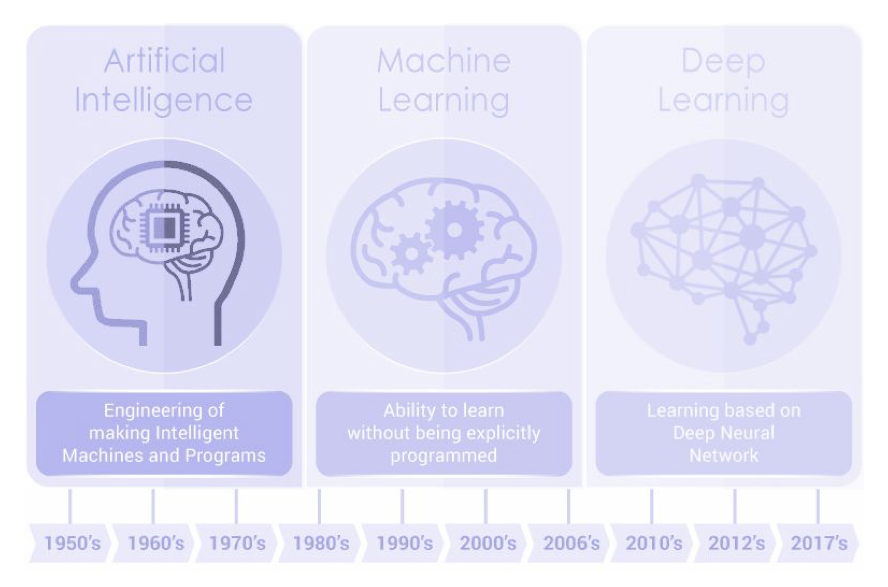
\includegraphics[width=0.7\textwidth]{../img/AI_ML_DL_1}
    \caption{Artificial Intelligence, Machine Learning and Deep Learning}
\end{figure}

It immediately becomes clear that deep learning is now the most
studied field(even if the idea of neural networks on its own is quite
old) of the entire artificial intelligence area and is also the
most promising one. In fact, most systems nowadays that apply some
kind of machine learning are actually based on deep learning models.
Furthermore, to understand even more deeply the relationships between
the three areas mentioned above, the next image could be useful:

\vspace{3mm}

\begin{figure}[h]
    \centering
    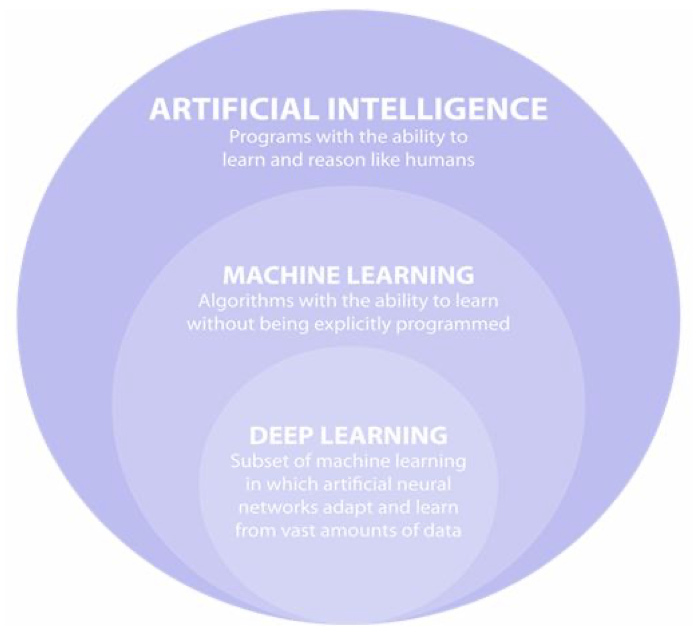
\includegraphics[width=0.4\textwidth]{../img/AI_ML_DL_2}
    \caption{Artificial Intelligence, Machine Learning and Deep Learning}
\end{figure}

\newpage

So, as the above images suggest, deep learning is the most recent
actually working accomplishment of machine learning and artificial
intelligence in general, which allows constructing complex and efficient
machine learning models that are based on the so-called artificial
neural networks, which adapt and learn from particularly large amounts
of data. These neural networks actually consist of several layers of
nodes between input and output that apply, instead of using the feature
extrapolation process, a hierarchical processing so that the network
itself automatically learns a mapping between the initial raw data and
the final output. In fact, in order to produce this mapping, some form
of representation of the input data is computed on each individual layer,
with the abstraction gradually increasing(i.e.\ from particular details
to general concepts) by aggregating the information from the lowest
layers near the input layer towards the highest layers near the output
layer. A summary of this process can be seen in the image below:

\vspace{5mm}

\begin{figure}[h]
    \centering
    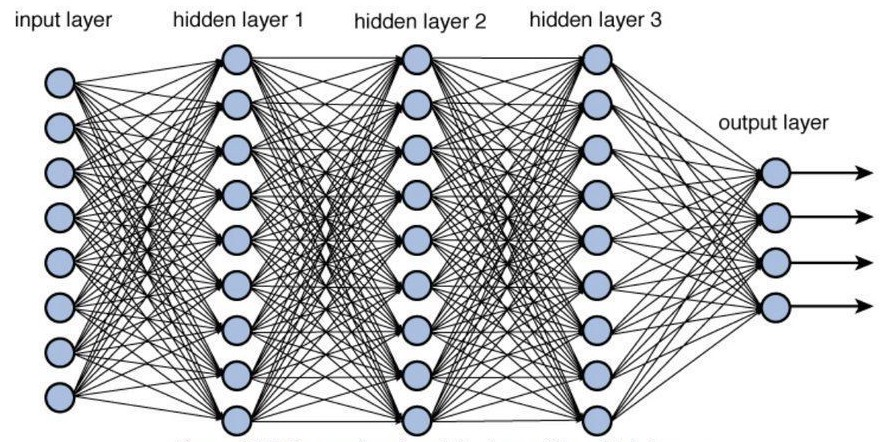
\includegraphics[width=0.7\textwidth]{../img/DNN}
    \caption{Deep Neural Network}
\end{figure}

\vspace{5mm}

At this point, it is worth mentioning some definitions of artificial
intelligence and deep learning, provided by big experts in these areas:

\vspace{5mm}

\begin{quoting}
    "Our ultimate objective is to make programs that learn from their
    experience as effectively as humans do."
\end{quoting}

\hspace{306pt}
\href{https://en.wikipedia.org/wiki/John_McCarthy_(computer_scientist)}{--- \underline{J. McCarthy(1958)}}

\vspace{5mm}

\begin{quoting}
    "Deep learning allows computational models that are composed of
    multiple processing layers to learn representations of data with
    multiple levels of abstraction"
\end{quoting}

\hspace{210pt}
\href{https://en.wikipedia.org/wiki/Geoffrey_Hinton}{--- \underline{G. Hinton}}
\href{https://en.wikipedia.org/wiki/Yann_LeCun}{--- \underline{Y. LeCun}}
\href{https://en.wikipedia.org/wiki/Yoshua_Bengio}{--- \underline{Y. Bengio}}

\newpage

The actual article about deep learning, its fundamental idea, and its
applications written by the fathers of deep learning(they won
the 2018 Turing Award for conceptual and engineering breakthroughs that
have made deep neural networks a critical component of computing) can be
found at this address:
\url{https://www.nature.com/articles/nature14539}.

At this point it is useful to mention some extremely important real-world
success stories that made deep learning so popular and so widely used:

\begin{itemize}
    \item \emph{Object Recognition}: This is a general machine
          learning task that is composed of other two machine learning
          tasks called Image Classification and Object Detection. The
          former consists in assigning to each object present in an
          image or in a frame of a video a label indicating the category
          to which that particular object belongs and a parameter
          indicating the degree of accuracy. The latter consists in
          assigning the position of that particular object by indicating
          the so-called bounding box, which defines the rectangular
          boundaries of where the object is located. The first actually
          working deep learning system that solves this general task on
          the dataset called ImageNet was created in 2012.
          Furthermore, in 2015, the error rate of another system on the
          same dataset has decreased to the level of a human being,
          which once again underlines the power of deep learning.
    \item \emph{Image Captioning}: This is a natural extension of
          Image Classification and a much more challenging task, which
          consists in assigning a textual description to an image or to
          a frame of a video. The first actually working deep learning
          system that solves this kind of task was created in 2015 and
          an excellent example of a similar system can be seen
          \href{https://www.youtube.com/watch?v=8BFzu9m52sc}{\underline{in this youtube video}}.
          Nowadays the systems that solve this kind of task have been
          further improved in performance.
    \item \emph{Image Synthesis}: This is another machine learning task
          that consists in automatically generating plausible images
          associated with the sketch of a scene passed as input. Such a
          system has been successfully developed by Nvidia.
    \item \emph{Speech Recognition}: This a self-explanatory machine
          learning task that has been studied for years and has been
          significantly improved in performance by using some deep
          learning techniques starting from 2009.
    \item \emph{Neural Machine Translation}: This a machine learning
          task that consists in translating sentences from one language
          to another and that has also been significantly improved in
          performance by using some deep learning approaches starting
          from 2014.
    \item \emph{Real-Time Voice Translation}: This is a machine learning
          task that consists in translating a person's speech in
          real-time by generating an artificial voice that speaks in the
          target language. An excellent example of a system that performs
          this kind of task can be seen
          \href{https://www.youtube.com/watch?v=Nu-nlQqFCKg}{\underline{in this youtube video}}.
    \item \emph{AlphaGO}: This is the aforementioned program that has
          been developed by the Google DeepMind group with the purpose
          of predicting the best future moves in an ancient Chinese game
          called Go and that has actually beaten the best world player
          at Go. An interesting fact is that a movie has been made about
          this story and the trailer can be seen
          \href{https://www.youtube.com/watch?v=8tq1C8spV_g}{\underline{in this youtube video}}.
\end{itemize}

\newpage

To conclude this subsection it is mandatory to mention the main reasons
why deep learning has only come into play in the last few years:

\begin{itemize}
    \item \emph{Flood of available data}: Nowadays the amount of data
          available is extremely large.
    \item \emph{Increased computational power}: There have been
          continuous improvements in hardware manufacturing that
          have made it possible to produce devices with a more powerful
          computational ability. In fact, an extremely important role
          for processing in the field of machine learning is played by
          GPUs.
    \item \emph{Research Development}: There are a lot of new machine
          learning algorithms and theory developed by researchers.
    \item \emph{Industry Involvement}: There is much more interest and
          support provided by companies, such as OpenAI, DeepMind and
          many others.
\end{itemize}